\section{Database Design}

\subsection{Data Model}
% -------------------------------------------------
\subsubsection*{Entity-Relationship Diagram (ERD)}

The ER model identifies the core entities required to streamline hospital operations and improve patient care. The system is built around five primary entities
\begin{itemize}
    \item \textbf{Patients:} Represents the individuals who receive medical services
    \item \textbf{Doctors:} Represents the medical professionals providing care
    \item \textbf{Departments:} Represents the organizational structure of the hospital
    \item \textbf{Appointments:} Represents the scheduled interactions between patients and doctors
    \item \textbf{Invoices:} Represents the financial transactions associated with patient visits
    \item \textbf{AuditLog:} Represents the system log recording automated data modifications
\end{itemize}

Key Relationships
\begin{itemize}
    \item \textbf{Departments to Doctors (1:N):} One department employs multiple doctors, but each doctor is assigned to exactly one department
    \item \textbf{Patients to Appointments (1:N):} A single patient can schedule multiple appointments over time
    \item \textbf{Doctors to Appointments (1:N):} A doctor can be assigned to multiple appointments with different patients
    \item \textbf{Patients to Invoices (1:N):} Each visit or service results in an invoice issued to a specific patient
\end{itemize}

\begin{figure}[H]
    \centering
    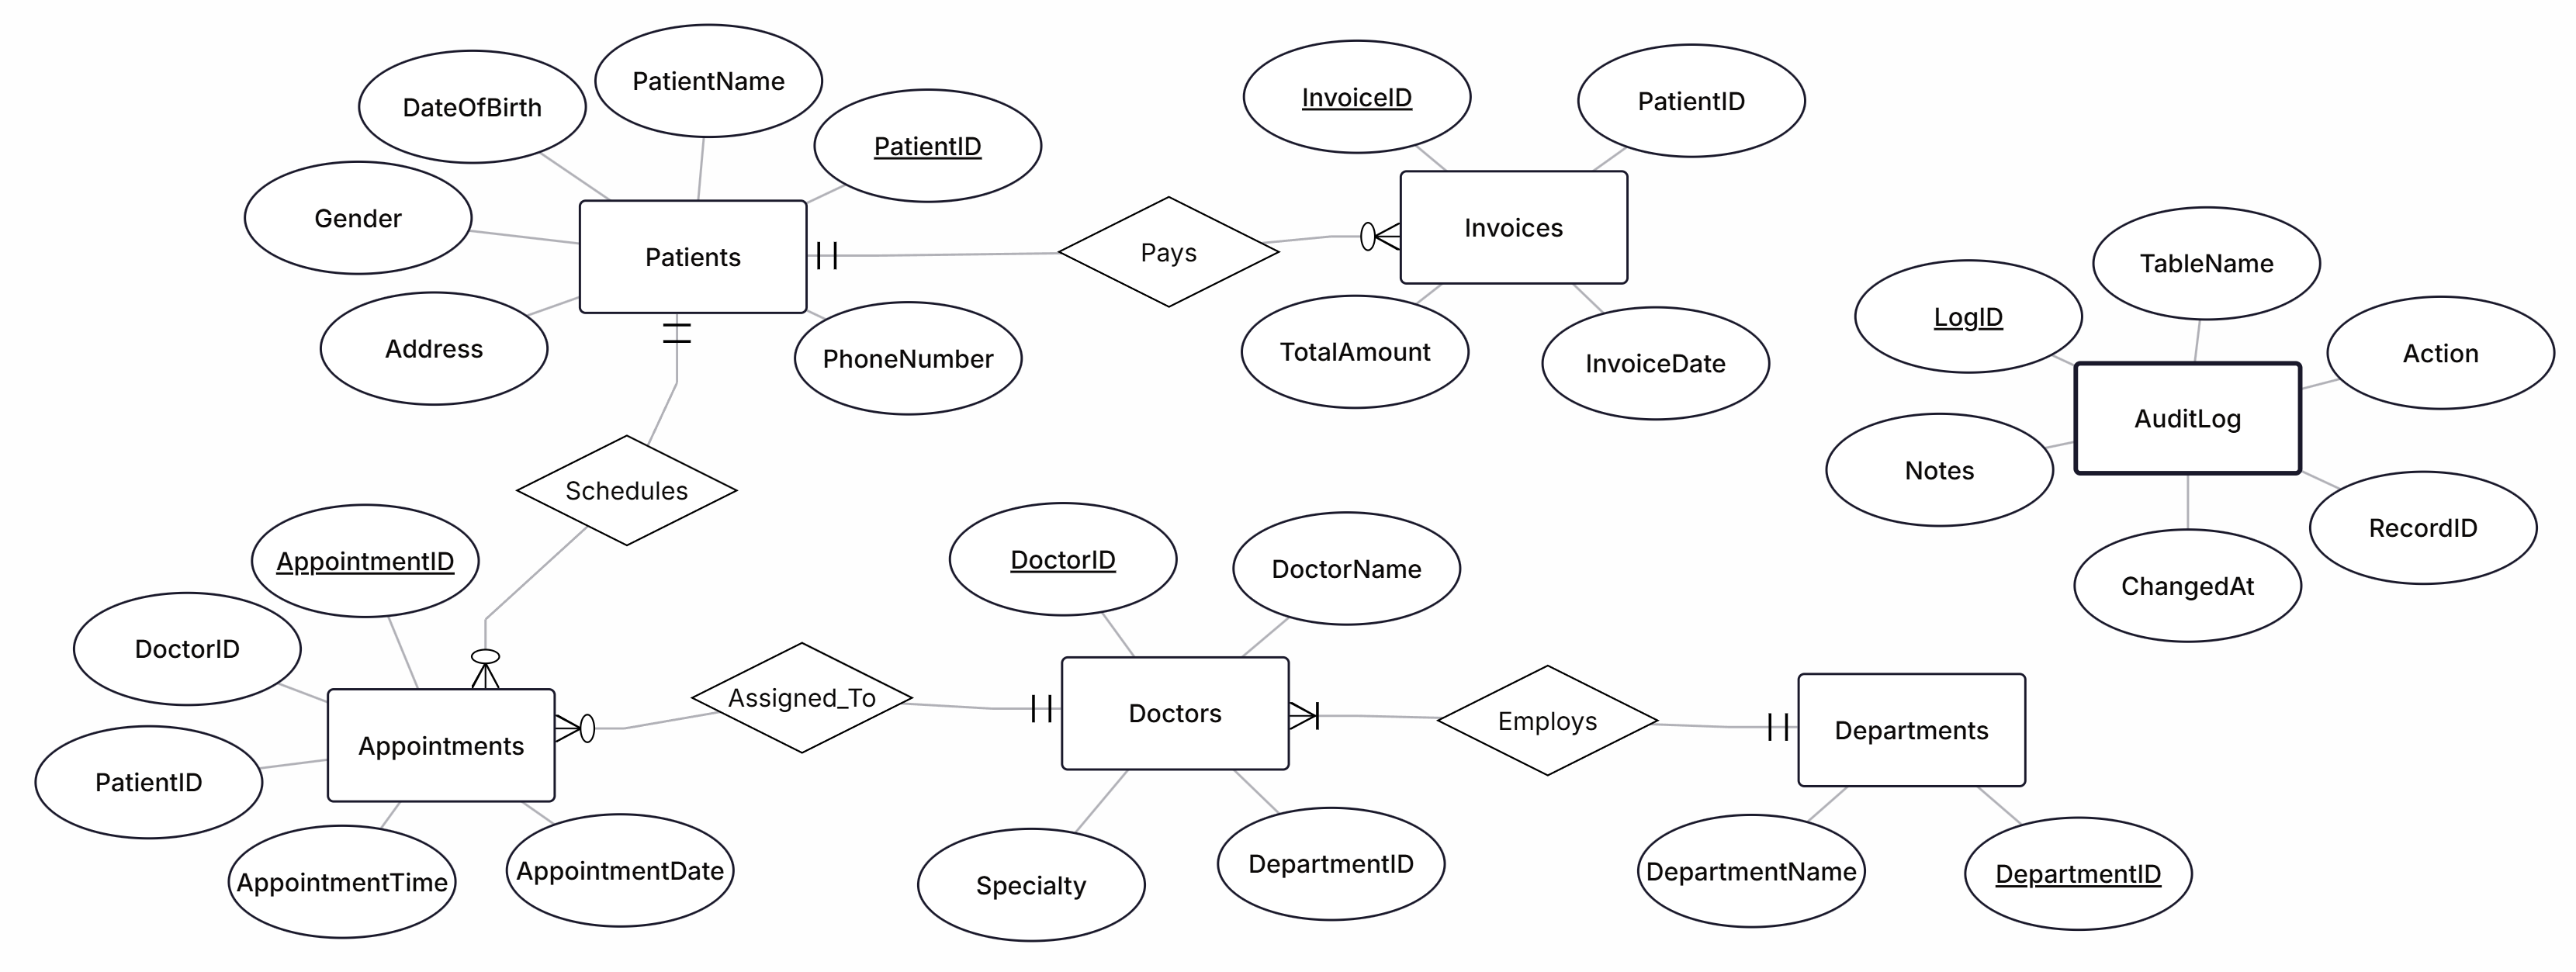
\includegraphics[width=1\textwidth]{Images/erdplus.png}
    \caption{ER Diagram}
    \label{fig:erd}
\end{figure}
% -------------------------------------------------
\subsubsection*{Relational Database Schema}

The conceptual ERD was converted into a relational schema to ensure data integrity and minimize redundancy. This logical model clearly defines the Primary Keys (PK), Foreign Keys (FK), and constraints required for a robust system.
\begin{itemize}
    \item \textbf{Primary Keys (PK):} Each table utilizes a unique identifier (e.g., \texttt{PatientID}, \texttt{DoctorID}) to ensure that every record can be uniquely retrieved
    \item \textbf{Foreign Keys (FK):} These keys establish the links between tables, such as \texttt{DepartmentID} in the \texttt{Doctors} table, which enforce referential integrity between staff and their respective departments
    \item \textbf{Data Integrity:} Constraints such as \texttt{NOT NULL} for names and dates, and specific data types like \texttt{DECIMAL(10, 2)} for financial amounts, ensure that the data remains accurate and reliable for reporting.
\end{itemize}

\begin{figure}[H]
    \centering
    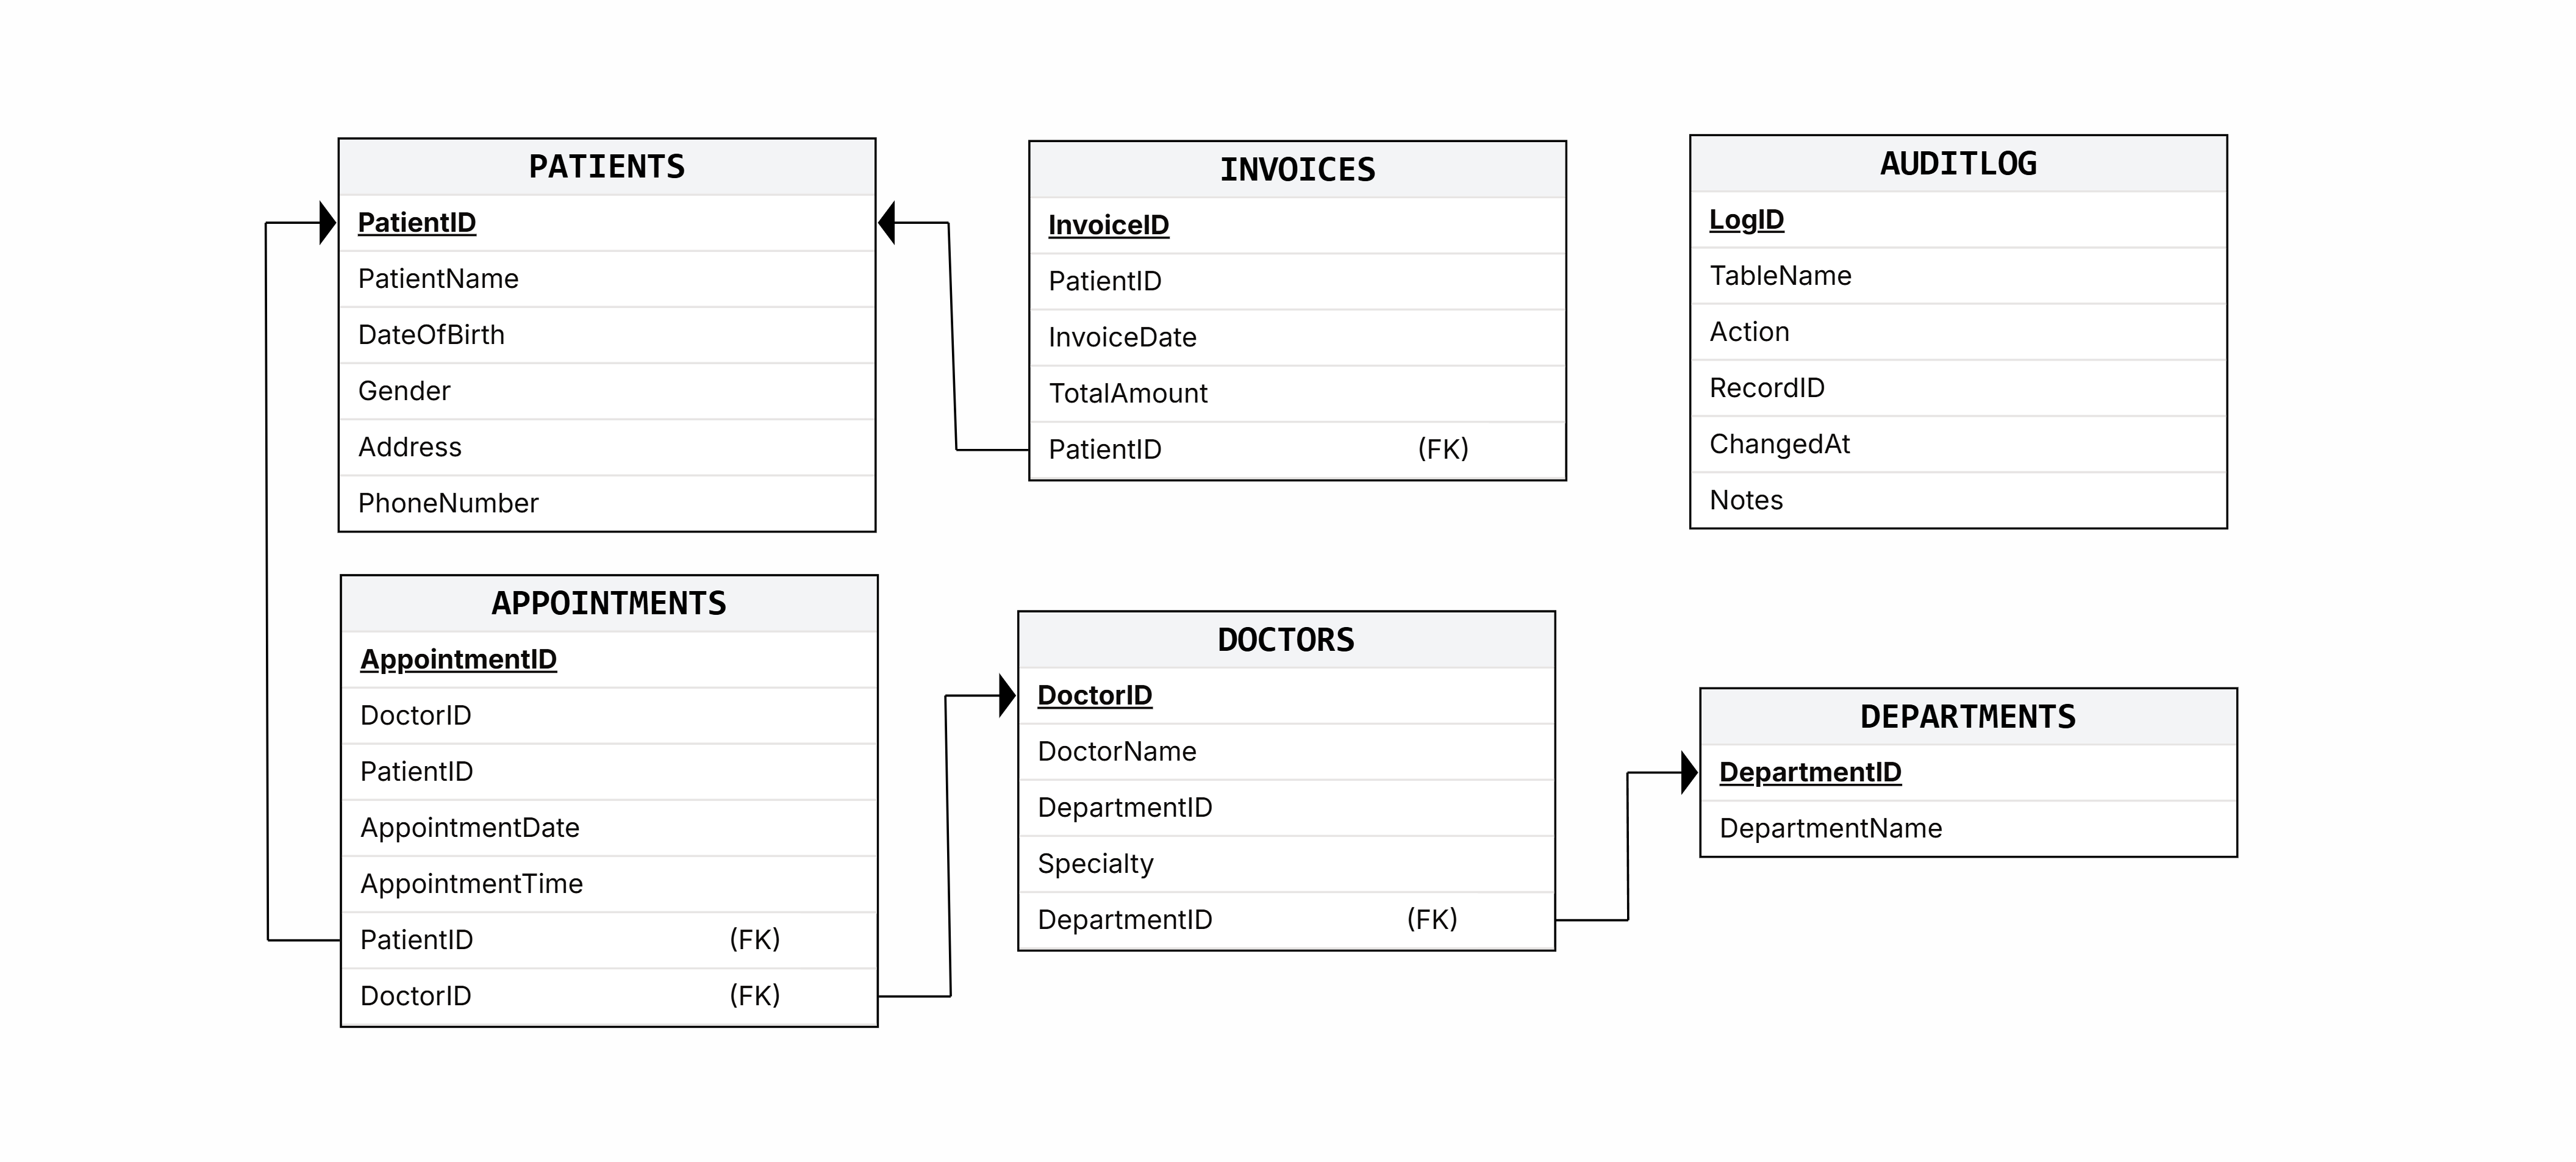
\includegraphics[width=0.9\textwidth]{Images/relational_diagram.png}
    \caption{Relational Schema}
    \label{fig:relational_diagram}
\end{figure}

% -------------------------------------------------
\subsection{Table Structures}

\subsubsection*{Patients}
This table serves as the central repository for personal information, storing contact details, demographic data, and birth dates for all individuals receiving care. It also tracks the date of the most recent payment made by each patient.
\begin{figure}[H]
    \centering
    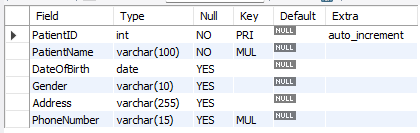
\includegraphics[width=0.6\textwidth]{Images/describe_patients.png}
    \caption{\texttt{DESCRIBE Patients} table}
    \label{fig:descirbe_patients}
\end{figure}

\subsubsection*{Doctors}
This table contains detailed profiles for medical practitioners, including their full names and specific areas of medical specialty. It also links each doctor to a specific department to maintain organizational structure.
\begin{figure}[H]
    \centering
    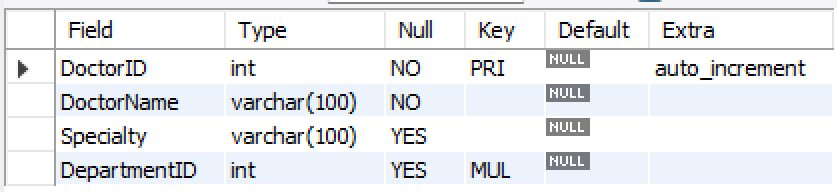
\includegraphics[width=0.8\textwidth]{Images/describe_doctors.png}
    \caption{\texttt{DESCRIBE Doctors} table}
    \label{fig:descirbe_doctors}
\end{figure}

\subsubsection*{Departments}
This table defines the various organizational units within the healthcare facility using unique identification codes and department names. It serves as a foundational classification level for organizing doctors and hospital resources.
\begin{figure}[H]
    \centering
    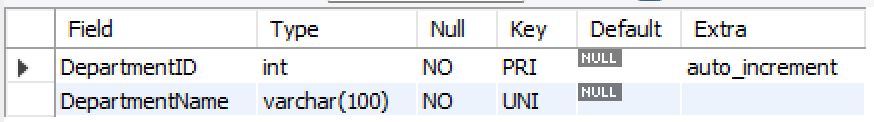
\includegraphics[width=0.8\textwidth]{Images/describe_departments.png}
    \caption{\texttt{DESCRIBE Departments} table}
    \label{fig:descirbe_departments}
\end{figure}

\subsubsection*{Appointments}
This table stores scheduled medical visits, tracking the specific date, time, and status of meetings between doctors and patients. It utilizes foreign keys to link individual patient records with their assigned medical professionals.
\begin{figure}[H]
    \centering
    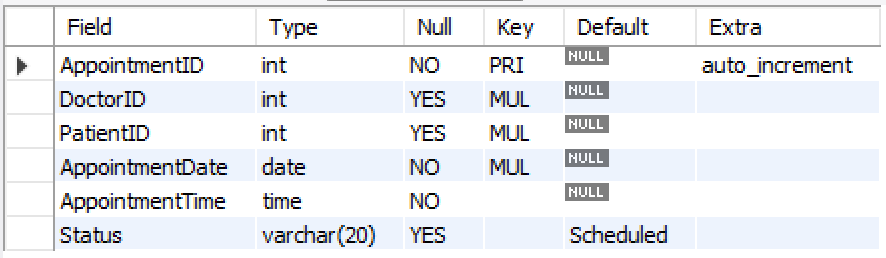
\includegraphics[width=0.8\textwidth]{Images/describe_appointments.png}
    \caption{\texttt{DESCRIBE Appointments} table}
    \label{fig:descirbe_appointments}
\end{figure}

\subsubsection*{Invoices}
This table manages financial transactions by recording the total amount billed, the issue date, and the current payment status for medical services. Each invoice is directly associated with a specific patient to track their financial history.
\begin{figure}[H]
    \centering
    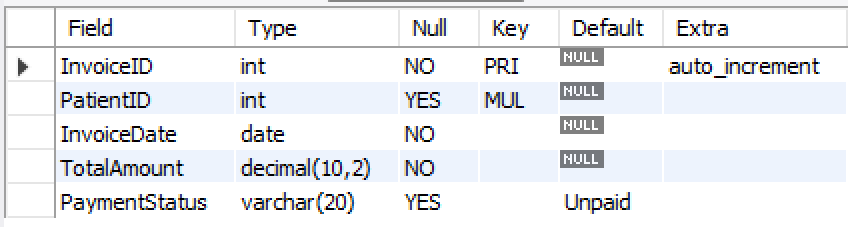
\includegraphics[width=0.8\textwidth]{Images/describe_invoices.png}
    \caption{\texttt{DESCRIBE Invoices} table}
    \label{fig:descirbe_invoices}
\end{figure}

\subsubsection*{AuditLog}
This table maintains a chronological record of system modifications, capturing the specific action taken, the affected table, and a precise timestamp. It is designed for monitoring data changes and includes a notes field for additional context regarding each entry.
\begin{figure}[H]
    \centering
    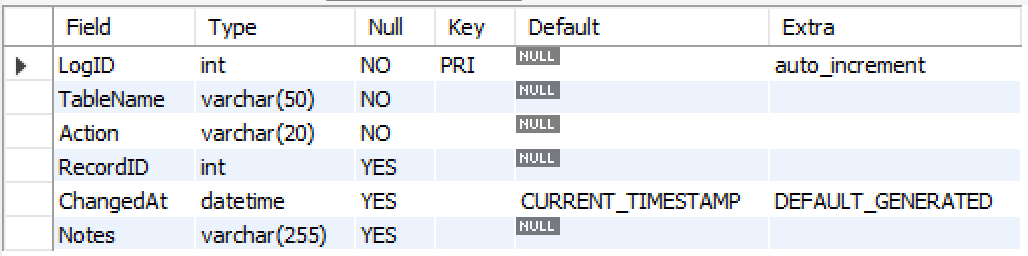
\includegraphics[width=0.8\textwidth]{Images/describe_auditlog.png}
    \caption{\texttt{DESCRIBE AuditLog} table}
    \label{fig:descirbe_auditlog}
\end{figure}